\chapter{Companies and Financial Accounting}
\section{Companies}
\subsection{What is a company?}
A company is a legal entity (``personality'') that can issue contracts, enter into agreements or contracts, assume obligations, incur and pay debts, sue and be sued in its own right, and be held responsible for its own actions. There are three main types of companies in the UK:
\begin{enumerate}
    \item A sole trader
    \item A partnership
    \item A limited liability company
\end{enumerate}
\subsubsection{Sole trader}
A sole trader:
\begin{itemize}
    \item Runs their own business as an individual
    \item Keeps all of the net profits
    \item Is personally responsible for any losses their business makes (unlimited liability)
\end{itemize}
\subsubsection{Partnership}
A partnership:
\begin{itemize}
    \item Involves two or more partners who share responsibility for the business
    \item Keeps all of the net profits (jointly)
    \item Is jointly responsible for any losses their business makes (joint unlimited liability)
    \item A partner does not have to be an actual person. For example, a limited company counts as a `legal person' and can also be a partner
\end{itemize}
\subsubsection{Limited liability company}
A limited liability company that is ``limited by shares'' or ``limited by guarantee.''

Limited by shares:
\begin{itemize}
    \item Usually businesses that make a profit
          \begin{itemize}
              \item is legally separate from those who run it (limited liability)
              \item has shares and shareholders
              \item retains net profits
          \end{itemize}
\end{itemize}

Limited by guarantee:
\begin{itemize}
    \item Usually businesses that are ``not for profit''
          \begin{itemize}
              \item is legally separate from those who run it (limited liability)
              \item has guarantors and a ``guaranteed amount''
              \item invests profits it makes back into the company
          \end{itemize}
\end{itemize}
\subsection{Structure of a limited liability company limited by shares}
\begin{figure}[H]
    \centering
    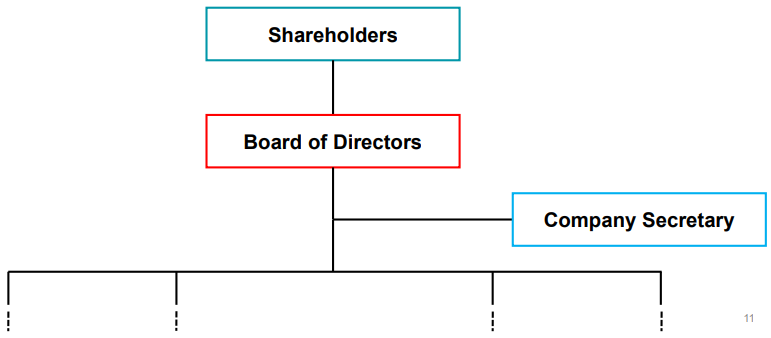
\includegraphics[width = \textwidth]{./img/figure26.png}
    \caption{Structure of a limited liability company limited by shares.}
\end{figure}
\subsection{What is a shareholder?}
\begin{itemize}
    \item Shareholders own a limited liability company limited by shares
    \item They have no day-to-day duties related to the company's operation
    \item Each shareholder owns a fraction of the company (and has corresponding voting power) proportional to their shareholding (investment)
    \item The liability of shareholders is limited to their original investment
    \item The company's profits are paid to shareholders as share dividend
\end{itemize}
\subsection{What is the board of directors?}
\begin{itemize}
    \item The board of directors is elected by the shareholders at the Annual General Meeting (AGM) to run the company.
          \begin{itemize}
              \item Directors may also be shareholders (but not necessarily)
              \item The shareholders can vote to appoint or sack individual board of directors members
          \end{itemize}
    \item The board of directors files the company's audited accounts (legal requirement)
    \item The board of directors report to the shareholders at the AGM (legal requirement)
    \item The board of directors is controller by the Chairman of the Board
    \item The board of directors can appoint or sack the Chief Executive Officer (CEO - responsible for day-to-day running)
\end{itemize}
\subsection{What is a company secretary?}
The company secretary ensures the smooth administration of the company. The company secretary is responsible for:
\begin{itemize}
    \item Making sure the company stays within the law
    \item Making sure the company maintains proper record books and accounts
    \item Providing strategic advice to the board of directors (sometimes)
\end{itemize}
The company secretary may or may not be a member of the board of directors.
\subsection{Limited liability company}
A limited liability company that is ``limited by shares'' can be public or private.

Private Limited Company (Ltd.):
\begin{itemize}
    \item Share ownership is controlled
          \begin{itemize}
              \item is owned privately
              \item only one director is required
              \item have nine months to file their annual accounts
              \item a company secretary is not legally required
          \end{itemize}
\end{itemize}

Public Limited Company (PLC):
\begin{itemize}
    \item Share ownership is NOT controlled
          \begin{itemize}
              \item company shares can be bought and sold publically on the open market (a stock exchange)
              \item two directors are required
              \item have six months to file their annual accounts
              \item a company secretary is legally required
          \end{itemize}
\end{itemize}